    
    
    
    

    

    \hypertarget{instruction-if-et-fonction-def}{%
\section{\texorpdfstring{Instruction \texttt{if} et fonction
\texttt{def}}{Instruction if et fonction def}}\label{instruction-if-et-fonction-def}}

    \hypertarget{exercice---niveau-basique}{%
\subsection{Exercice - niveau basique}\label{exercice---niveau-basique}}

    \hypertarget{fonction-de-divisibilituxe9}{%
\subsubsection{Fonction de
divisibilité}\label{fonction-de-divisibilituxe9}}

    \begin{Verbatim}[commandchars=\\\{\},frame=single,framerule=0.3mm,rulecolor=\color{cellframecolor}]
{\color{incolor}In [{\color{incolor}1}]:} \PY{c+c1}{\PYZsh{} chargement de l\PYZsq{}exercice}
        \PY{k+kn}{from} \PY{n+nn}{corrections}\PY{n+nn}{.}\PY{n+nn}{exo\PYZus{}divisible} \PY{k}{import} \PY{n}{exo\PYZus{}divisible}
\end{Verbatim}


    L'exercice consiste à écrire une fonction baptisée \texttt{divisible}
qui retourne une valeur booléenne, qui indique si un des deux arguments
est divisible par l'autre.

Vous pouvez supposer les entrées \texttt{a} et \texttt{b} entiers et non
nuls, mais pas forcément positifs.

    \begin{Verbatim}[commandchars=\\\{\},frame=single,framerule=0.3mm,rulecolor=\color{cellframecolor}]
{\color{incolor}In [{\color{incolor}2}]:} \PY{k}{def} \PY{n+nf}{divisible}\PY{p}{(}\PY{n}{a}\PY{p}{,} \PY{n}{b}\PY{p}{)}\PY{p}{:}
            \PY{l+s+s2}{\PYZdq{}}\PY{l+s+s2}{\PYZlt{}votre\PYZus{}code\PYZgt{}}\PY{l+s+s2}{\PYZdq{}}
\end{Verbatim}


    Vous pouvez à présent tester votre code en évaluant ceci, qui écrira un
message d'erreur si un des jeux de test ne donne pas le résultat
attendu.

    \begin{Verbatim}[commandchars=\\\{\},frame=single,framerule=0.3mm,rulecolor=\color{cellframecolor}]
{\color{incolor}In [{\color{incolor} }]:} \PY{c+c1}{\PYZsh{} NOTE}
        \PY{c+c1}{\PYZsh{} auto\PYZhy{}exec\PYZhy{}for\PYZhy{}latex has skipped execution of this cell}
        
        \PY{c+c1}{\PYZsh{} tester votre code}
        \PY{n}{exo\PYZus{}divisible}\PY{o}{.}\PY{n}{correction}\PY{p}{(}\PY{n}{divisible}\PY{p}{)}
\end{Verbatim}


    \hypertarget{exercice---niveau-basique}{%
\subsection{Exercice - niveau basique}\label{exercice---niveau-basique}}

    \hypertarget{fonction-duxe9finie-par-morceaux}{%
\subparagraph{Fonction définie par
morceaux}\label{fonction-duxe9finie-par-morceaux}}

    \begin{Verbatim}[commandchars=\\\{\},frame=single,framerule=0.3mm,rulecolor=\color{cellframecolor}]
{\color{incolor}In [{\color{incolor}3}]:} \PY{c+c1}{\PYZsh{} chargement de l\PYZsq{}exercice}
        \PY{k+kn}{from} \PY{n+nn}{corrections}\PY{n+nn}{.}\PY{n+nn}{exo\PYZus{}morceaux} \PY{k}{import} \PY{n}{exo\PYZus{}morceaux}
\end{Verbatim}


    On veut définir en Python une fonction qui est définie par morceaux~:

    \[
f: x \longrightarrow \left\{
\begin{array}{ll}
-x - 5          & \mbox{si } x \leqslant -5 \\
0               & \mbox{si } x \in [-5, 5]  \\
\frac{1}{5}x -1 & \mbox{si } x \geqslant 5  \\
\end{array}
\right.
\]

    \begin{Verbatim}[commandchars=\\\{\},frame=single,framerule=0.3mm,rulecolor=\color{cellframecolor}]
{\color{incolor}In [{\color{incolor}4}]:} \PY{c+c1}{\PYZsh{} donc par exemple}
        \PY{n}{exo\PYZus{}morceaux}\PY{o}{.}\PY{n}{example}\PY{p}{(}\PY{p}{)}
\end{Verbatim}


\begin{Verbatim}[commandchars=\\\{\},frame=single,framerule=0.3mm,rulecolor=\color{cellframecolor}]
{\color{outcolor}Out[{\color{outcolor}4}]:} <IPython.core.display.HTML object>
\end{Verbatim}
            
    \begin{Verbatim}[commandchars=\\\{\},frame=single,framerule=0.3mm,rulecolor=\color{cellframecolor}]
{\color{incolor}In [{\color{incolor}5}]:} \PY{c+c1}{\PYZsh{} à vous de jouer}
        
        \PY{k}{def} \PY{n+nf}{morceaux}\PY{p}{(}\PY{n}{x}\PY{p}{)}\PY{p}{:}
            \PY{k}{return} \PY{l+m+mi}{0} \PY{c+c1}{\PYZsh{} \PYZdq{}votre code\PYZdq{}}
\end{Verbatim}


    \begin{Verbatim}[commandchars=\\\{\},frame=single,framerule=0.3mm,rulecolor=\color{cellframecolor}]
{\color{incolor}In [{\color{incolor} }]:} \PY{c+c1}{\PYZsh{} NOTE}
        \PY{c+c1}{\PYZsh{} auto\PYZhy{}exec\PYZhy{}for\PYZhy{}latex has skipped execution of this cell}
        
        \PY{c+c1}{\PYZsh{} pour corriger votre code}
        \PY{n}{exo\PYZus{}morceaux}\PY{o}{.}\PY{n}{correction}\PY{p}{(}\PY{n}{morceaux}\PY{p}{)}
\end{Verbatim}


    \hypertarget{repruxe9sentation-graphique}{%
\subparagraph{Représentation
graphique}\label{repruxe9sentation-graphique}}

    L'exercice est terminé, mais nous allons maintenant voir ensemble
comment vous pourriez visualiser votre fonction.

Voici ce qui est attendu comme courbe pour \texttt{morceaux} (image
fixe)~: 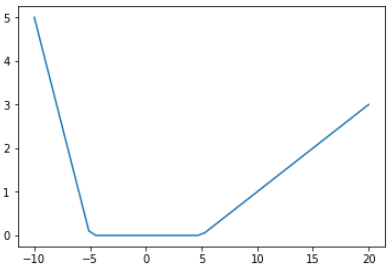
\includegraphics{media/morceaux.png}

    En partant de votre code, vous pouvez produire votre propre courbe en
utilisant \texttt{numpy} et \texttt{matplotlib} comme ceci~:

    \begin{Verbatim}[commandchars=\\\{\},frame=single,framerule=0.3mm,rulecolor=\color{cellframecolor}]
{\color{incolor}In [{\color{incolor}6}]:} \PY{c+c1}{\PYZsh{} on importe les bibliothèques}
        \PY{k+kn}{import} \PY{n+nn}{numpy} \PY{k}{as} \PY{n+nn}{np}
        \PY{k+kn}{import} \PY{n+nn}{matplotlib}\PY{n+nn}{.}\PY{n+nn}{pyplot} \PY{k}{as} \PY{n+nn}{plt}
\end{Verbatim}


    \begin{Verbatim}[commandchars=\\\{\},frame=single,framerule=0.3mm,rulecolor=\color{cellframecolor}]
{\color{incolor}In [{\color{incolor}7}]:} \PY{c+c1}{\PYZsh{} un échantillon des X entre \PYZhy{}10 et 20}
        \PY{n}{X} \PY{o}{=} \PY{n}{np}\PY{o}{.}\PY{n}{linspace}\PY{p}{(}\PY{o}{\PYZhy{}}\PY{l+m+mi}{10}\PY{p}{,} \PY{l+m+mi}{20}\PY{p}{)}
        
        \PY{c+c1}{\PYZsh{} et les Y correspondants}
        \PY{n}{Y} \PY{o}{=} \PY{n}{np}\PY{o}{.}\PY{n}{vectorize}\PY{p}{(}\PY{n}{morceaux}\PY{p}{)}\PY{p}{(}\PY{n}{X}\PY{p}{)}
\end{Verbatim}


    \begin{Verbatim}[commandchars=\\\{\},frame=single,framerule=0.3mm,rulecolor=\color{cellframecolor}]
{\color{incolor}In [{\color{incolor}8}]:} \PY{c+c1}{\PYZsh{} on n\PYZsq{}a plus qu\PYZsq{}à dessiner}
        \PY{n}{plt}\PY{o}{.}\PY{n}{plot}\PY{p}{(}\PY{n}{X}\PY{p}{,} \PY{n}{Y}\PY{p}{)}
        \PY{n}{plt}\PY{o}{.}\PY{n}{show}\PY{p}{(}\PY{p}{)}
\end{Verbatim}


    \begin{center}
    \adjustimage{max size={0.9\linewidth}{0.9\paperheight}}{w2-s6-x4-if-et-def_files/w2-s6-x4-if-et-def_22_0.png}
    \end{center}
    { \hspace*{\fill} \\}
    

    % Add a bibliography block to the postdoc
    
    
    
